\chapter{Platform Architecture and Implementation}
\label{chap:platform}
\emergencystretch=3em\relax

This chapter explains how the scoring engine presented in Chapter~\ref{chap:scoring-engine} is embedded in a complete, secure and deployable application. The engine itself is treated as a black box here, frozen, audited and pure by construction (principle P1, Chapter~\ref{chap:method}); what this chapter narrates is everything that surrounds it. Section~\ref{sec:platform-architecture} lays out the overall layering. Sections~\ref{sec:platform-backend} and \ref{sec:platform-frontend} cover the backend and the frontend in turn. Section~\ref{sec:platform-auth-security} is the largest of the six, it details the authentication model and the security measures built around it. Section~\ref{sec:platform-local-ai} explains how a local language model turns a computed result into a narrative without ever touching the score. Section~\ref{sec:platform-networking} closes the chapter with the operational choices, and one particular problem, that kept the stack working across a virtual machine boundary during development.

% --------------------------------------------------------------
\section{Overall architecture}
\label{sec:platform-architecture}

The platform is organised in four layers, shown in Figure~\ref{fig:platform-architecture-layers} (Appendix~\ref{app:figures}). The frontend (Section~\ref{sec:platform-frontend}) is a Next.js client that renders the questionnaire and the results dashboard and never enforces access on its own. The backend API (Section~\ref{sec:platform-backend}) is a FastAPI application that exposes the HTTP surface, applies authentication and authorisation before any handler runs, and persists raw user input in SQLite. Between the API and the engine sits a single translation module, \texttt{scoring\_\allowbreak bridge.\allowbreak py}, described below. Downstream of the engine, a local AI layer (Section~\ref{sec:platform-local-ai}) reads the computed result and produces a narrative, without ever touching the score itself.

This separation is not incidental. It extends to the rest of the application the same discipline that governs the engine's own design, and it rests on principle P4 (Chapter~\ref{chap:method}): the referential in \texttt{referential.\allowbreak yaml} is the single source of truth for the business rules, never duplicated in the database schema or in the frontend code.

\subsection{Why the DB layer and the engine layer stay separate}

The SQLAlchemy models that persist a questionnaire, \texttt{Answer} and \texttt{BPAnnotation}, store raw inputs only, and I kept them deliberately distinct from the engine's own Pydantic input models. A \texttt{question\_\allowbreak id} or a \texttt{bp\_\allowbreak id} is a plain string in the database, not a foreign key into the framework, because the framework lives in \texttt{referential.\allowbreak yaml} and not in the schema (P4). The database module never imports the engine, and the engine never imports the database module.

I considered folding the two together, since both ultimately describe the same questionnaire, but rejected it: coupling persistence to the engine's models would let an unrelated schema change silently alter what the engine scores, and would make the engine depend on the database, which breaks the purity and the standalone testability that Chapter~\ref{chap:scoring-engine} establishes as non-negotiable. Keeping two layers costs one extra translation step, but it means a migration can evolve the schema without ever touching the scoring logic, and the engine's 70 tests keep running against nothing but Pydantic objects, with no database in sight.

\subsection{The single translation seam: \texttt{scoring\_\allowbreak bridge.\allowbreak py}}

That one extra translation step lives entirely in \texttt{app/\allowbreak scoring\_\allowbreak bridge.\allowbreak py}, the only module in the codebase that imports both the ORM models and the engine's input models. \texttt{build\_\allowbreak assessment\_\allowbreak input} maps a stored \texttt{Assessment}, with its answers and BP annotations eagerly loaded, to the engine's \texttt{Assessment\allowbreak Input}, dropping any answer row that is structurally incomplete. A companion function, \texttt{missing\_\allowbreak answers}, precomputes the full list of gaps in one pass, so the API can report every missing answer to the user at once instead of stopping at the first one the engine happens to trip over.

No scoring rule is reimplemented in this module. Concentrating the translation in one place is what makes the separation above actually hold in practice: the engine stays pure and unaware of the database, and the storage layer stays unaware of scoring. A dedicated test, \texttt{score\_\allowbreak test.\allowbreak py}, cross-checks that seam end to end, from a stored assessment to a final score.

% --------------------------------------------------------------
\section{Backend}
\label{sec:platform-backend}

The backend is a FastAPI application backed by SQLite through an asynchronous SQLAlchemy 2.x stack, with Alembic managing every schema change. \texttt{app/\allowbreak database.\allowbreak py} builds the async engine (\texttt{sqlite+aiosqlite}, defaulting to a local \texttt{crisis\_\allowbreak maturity.\allowbreak db} file) and a single declarative base. I settled on this combination for a minimum viable product (MVP) with a short runway to the deadline: SQLite needs no separate infrastructure to run or to demonstrate, the asynchronous stack matches FastAPI's own request model rather than blocking it, and it pre-empts a planned migration to PostgreSQL later, which should in principle come down to the connection string alone, though Chapter~\ref{chap:impact} notes that this has not been attempted. Alembic from the first commit means the schema is versioned and reproducible, \texttt{alembic upgrade head} rebuilds a fresh database from nothing, instead of relying on an implicit \texttt{create\_\allowbreak all}.

\subsection{Data model and persistence}

Five models carry the application's state: \texttt{User}, \texttt{Organization}, \texttt{Assessment}, \texttt{Answer} and \texttt{BPAnnotation}. An \texttt{Assessment} belongs to a \texttt{User} and, optionally, an \texttt{Organization}, and carries the \texttt{referential\_\allowbreak version} it was scored against together with a status (\texttt{in\_\allowbreak progress} or \texttt{submitted}). Each \texttt{Answer} row stores one declared maturity level and its evidence type for one question, and each \texttt{BPAnnotation} row stores whether a best practice was marked not applicable, with a justification. A unique constraint on \texttt{(assessment\_\allowbreak id, question\_\allowbreak id)} and on \texttt{(assessment\_\allowbreak id, bp\_\allowbreak id)} keeps an assessment from ever holding two conflicting answers to the same question, and indexes on \texttt{Assessment.\allowbreak user\_\allowbreak id}, \texttt{organization\_\allowbreak id} and \texttt{status} keep the per-owner listing queries (Section~\ref{sec:platform-auth-security}) cheap. The initial migration, \texttt{b76d1f7e713a\_\allowbreak initial\_\allowbreak schema.\allowbreak py}, creates all five tables at once with these constraints already in place.

The \texttt{User.\allowbreak role} field started, at this stage of the project, with an \texttt{anonymous} default alongside \texttt{respondent}, \texttt{consultant} and \texttt{admin}. Section~\ref{sec:platform-auth-security} explains where that default came from and how it disappeared, behind the same dependency signature, without touching this schema.

\subsection{The score is computed on the fly, never stored}

\texttt{POST /\allowbreak api/\allowbreak assessments/\allowbreak \{id\}/\allowbreak score} runs the engine and returns the serialised \texttt{Assessment\allowbreak Result}, but it never writes it back to the database, and it leaves the assessment's status untouched. I considered caching the result for performance, since recomputation is not free. A stored score can drift from its own inputs the moment an answer is edited or the referential is bumped to a new version, though, and a drifted score is exactly what the engine's determinism guarantee (P1, Chapter~\ref{chap:method}) exists to prevent. The result stays fully reproducible from the raw inputs plus the referential version, so recomputing it on every request is the only option that cannot go stale; a cache, if one is ever needed, would have to sit on top of that recomputation, never replace it. The same endpoint keeps user errors out of the \texttt{5xx} range: an incomplete questionnaire or an engine validation failure (\texttt{NAValidation\allowbreak Error}) is surfaced as a \texttt{422}, not a server error.  The full HTTP surface this backend exposes, with the access control applied to each route, is tabulated in Table~\ref{tab:backend-api-endpoints}, Appendix~\ref{app:tables}.

% --------------------------------------------------------------
\section{Frontend}
\label{sec:platform-frontend}

The frontend is a single Next.js 14 client using the App Router, written in strict TypeScript (no \texttt{any}, unused variables treated as errors by ESLint), styled with Tailwind and shadcn/ui, and charted with Recharts. \texttt{lib/\allowbreak api.\allowbreak ts} wraps every call to the backend behind a thin fetch helper that always sends \texttt{credentials:\allowbreak  'include'}, so the session cookie set up in Section~\ref{sec:platform-auth-security} rides along automatically; Section~\ref{sec:platform-networking} comes back to a problem that this same setting caused once the frontend and the backend stopped sharing an origin.

The independent audit of the scoring engine (Chapter~\ref{chap:scoring-engine}) had flagged one pitfall ahead of time for whoever built the frontend: \texttt{Consistency\allowbreak Penalty.\allowbreak bp\_\allowbreak pair} is a Python \texttt{tuple[str, str]} in the engine, but it serialises to a plain JSON array once it crosses \texttt{GET /\allowbreak api/\allowbreak referential}, so a strict TypeScript type has to read it as \texttt{[string, string]} and not the more natural \texttt{string[]}, or the typing guarantee is lost silently. The frontend honours this: \texttt{bp\_\allowbreak pair} is declared as the two-element tuple in \texttt{frontend/\allowbreak lib/\allowbreak assessment.\allowbreak ts}, not as \texttt{string[]}, and every consumer reads it positionally, \texttt{bp\_\allowbreak pair[0]} and \texttt{bp\_\allowbreak pair[1]} rather than iterating over it, so the anticipated pitfall never materialised in practice.

\subsection{A per-phase questionnaire with idempotent autosave}

The questionnaire is a per-phase flow, one screen per phase of the referential (Prevention, Preparedness, Response, Recovery), with best-practice-level N/A annotations, rather than one long form. Keeping each screen short was a deliberate choice against anti-pattern~9 (Chapter~\ref{chap:method}), and the four-phase split falls directly out of the referential's own structure, so the flow needed no separate design decision once the referential was loaded at startup. Saving an answer is idempotent by construction: the database enforces a unique constraint on the pair \texttt{(assessment\_\allowbreak id, question\_\allowbreak id)} (Section~\ref{sec:platform-backend}), so retrying the same save after a dropped connection cannot create a duplicate answer, it can only overwrite the previous value for that question.

\subsection{Results dashboard}

Once an assessment is complete, the results screen turns the computed \texttt{Assessment\allowbreak Result} into a dashboard: a radar chart across the four phases, a bar per best practice, and a single headline score with its maturity level, shown in Figure~\ref{fig:frontend-dashboard}.

\begin{figure}[ht!]
  \centering
  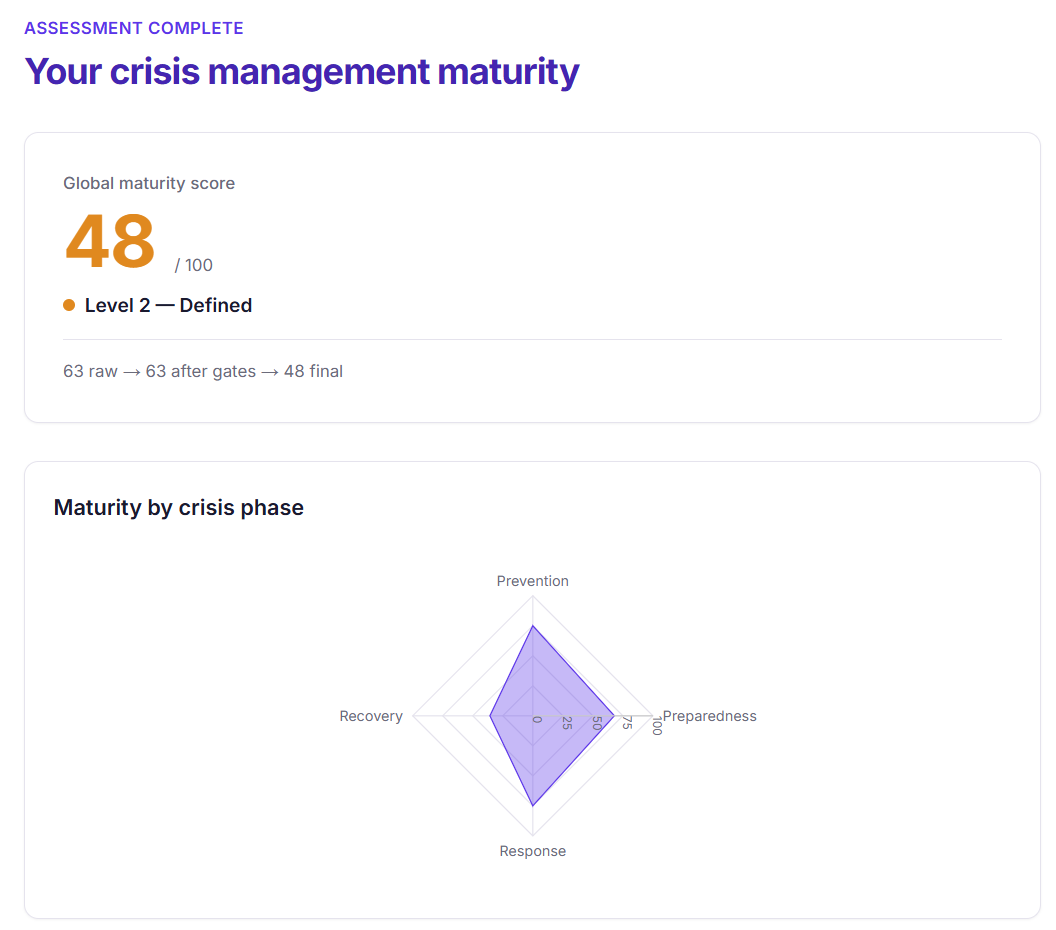
\includegraphics[width=0.72\textwidth]{figures/dashboard-score-radar.png}\\[3mm]
  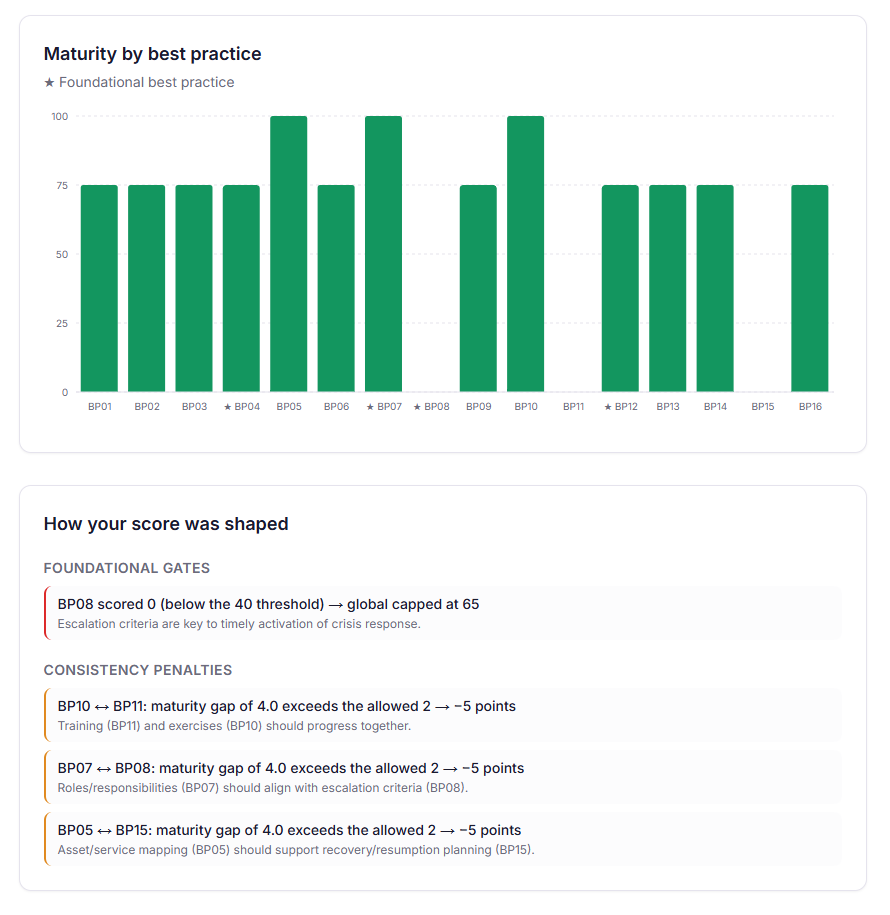
\includegraphics[width=0.72\textwidth]{figures/dashboard-bp-bars.png}
  \caption{Assessment results dashboard: global maturity score and radar chart by phase (top), bar chart by best practice with the foundational gates and consistency penalties that shaped the final score (bottom)}
  \label{fig:frontend-dashboard}
\end{figure}

\subsection{No duplicated framework content, one token layer for theming}

Every component that renders a question or a best-practice name fetches it from \texttt{GET /\allowbreak api/\allowbreak referential} rather than hardcoding it, the same P4 discipline (Chapter~\ref{chap:method}) applied to the frontend: the referential is read once, never copied into a component. Colour follows the same one-place principle, every colour in the interface lives in CSS custom properties in \texttt{app/\allowbreak globals.\allowbreak css}, so re-theming the whole application is a single-file edit. The palette itself is a violet-and-grey scheme inspired by Wavestone's identity, deliberately not copied from the official charter and using no Wavestone logo, which keeps the deliverable presentable to the company without misrepresenting a student project as an official Wavestone product.

\subsection{i18n: English only, no locale routing (for now)}

Text goes through \texttt{next-\allowbreak intl}, but the interface ships in English only, with no URL-prefixed locale routing such as \texttt{/\allowbreak en} or \texttt{/\allowbreak fr}. I considered adding routed locales from the start, since a consulting client base is not necessarily English-speaking, but rejected it as premature for a single-language MVP: every string already goes through a message key, so adding a second language later is a two-line change to a messages file, not a rewrite of any component. The cost of the full routing machinery is deferred until there is a second language to justify it.

None of this is a security boundary. The interface hides screens a user should not see and redirects an unauthenticated visitor to the login page; every protected call still stands on its own behind the checks described in Section~\ref{sec:platform-auth-security}, and a user who reaches an endpoint directly gets exactly the same 401, 403 or 404 the backend would have returned anyway.

% --------------------------------------------------------------
\section{Authentication and security}
\label{sec:platform-auth-security}

Real authentication did not appear all at once. From the first sprint, the backend already carried a full users, organisations and roles schema, and every route already depended on \texttt{Depends(get\_\allowbreak current\_\allowbreak user)}; at that stage the dependency was a stub that read an opaque session cookie and silently created an anonymous \texttt{User} row on first contact (principle P5, Chapter~\ref{chap:method}). The stub existed precisely so that real authentication could later replace one function behind a fixed signature, not force a schema migration or a rewrite of every route. This section covers what replaced it: the invitation cascade that turns an email address into an account, the session model, the roles and the per-owner access control built on top of them, and the concrete security measures that follow from treating a platform handling client organisations' maturity data as something that has to defend itself.

\subsection{Invitation cascade and account activation}

Accounts are never created directly. An admin or a consultant issues a single-use invitation bound to one email address and one role; the recipient turns it into an account by choosing a password at \texttt{POST /\allowbreak api/\allowbreak auth/\allowbreak accept}. I call this option B: an invitation link that leads to a chosen password, as opposed to a passwordless magic link that would log the user in directly. The backend never sends an email itself, \texttt{POST /\allowbreak api/\allowbreak auth/\allowbreak invitations} returns the clear token exactly once and a human relays it out of band, a sequence set out in Figure~\ref{fig:auth-invitation-cascade} in Appendix~\ref{app:figures}. I chose this over building an SMTP integration because the environment genuinely has none configured, and because the consulting workflow is human-driven anyway: a consultant already knows the client they are onboarding and can hand them a link directly. A pure magic link would have avoided a password entirely, but it gives no durable credential for a client who comes back a week later, so option B trades one extra step at signup for a normal login afterwards. The very first admin account is seeded the same way, by \texttt{backend/\allowbreak bootstrap\_\allowbreak admin.\allowbreak py}, which creates an admin invitation with \texttt{invited\_\allowbreak by} left \texttt{NULL}; every other account, including that first admin, is activated through the exact same \texttt{accept\_\allowbreak invitation} path, so there is only one place in the codebase that enforces the password policy and the bcrypt hashing described below.

Who may invite whom is fixed as well: an admin can invite an admin, a consultant or a respondent; a consultant can only invite a respondent; a respondent invites nobody. The role on an activated account comes from the invitation itself, never from the accept request, so a recipient has no way to hand themselves a higher role than the one they were invited with. Invitations are also single-use and time-bounded, a consumed token or an expired one cannot be replayed, which closes off both reusing an old link and leaving a leaked one usable indefinitely.

\subsection{Server-side sessions, not JWT}

Logging in, or accepting an invitation, opens a row in a \texttt{sessions} table and stores only the SHA-256 hash of an opaque random token; the clear token itself rides in an HttpOnly cookie, never reachable from JavaScript. \texttt{get\_\allowbreak current\_\allowbreak user} resolves that cookie to a session and then to a user on every request. The project brief mandated cookie sessions and ruled out JWT, and the case for it holds beyond the brief: a server-side store gives real revocation, logging out, or a future ``kill all sessions'' action, only has to delete the row, so a stolen or copied token dies immediately. A stateless JWT cannot do that without maintaining a blocklist, which is a server-side store by another name, so cookie sessions did not cost anything a JWT would have saved. Every session is also bounded by an \texttt{expires\_\allowbreak at}, regardless of whether it is ever explicitly revoked.

The cookie itself carries three attributes together: HttpOnly (unreachable from JavaScript, closing off token theft through XSS), SameSite=Lax (a first line of defence against CSRF), and Secure, configurable and required in production to stop the cookie riding over plain HTTP. Section~\ref{sec:platform-networking} returns to what SameSite actually cost during development, once the frontend and the backend stopped being the same origin.

\subsection{A problem encountered: passlib versus bcrypt}

The first attempt at password hashing went through \texttt{passlib}, the usual wrapper library, and it broke immediately: \texttt{passlib} 1.7.4 is unmaintained and crashes against \texttt{bcrypt} 5.x, because it inspects a \texttt{\_\allowbreak \_\allowbreak about\_\allowbreak \_\allowbreak .\allowbreak \_\allowbreak \_\allowbreak version\_\allowbreak \_\allowbreak } attribute that no longer exists on the newer package. Rather than pin an old, unmaintained \texttt{bcrypt} version to keep \texttt{passlib} happy, I called \texttt{bcrypt} directly, \texttt{hashpw} and \texttt{checkpw}, and kept that call inside one small, unit-tested module, \texttt{app/\allowbreak core/\allowbreak security.\allowbreak py}. The session and invitation tokens, which are high-entropy random values rather than user-chosen passwords, are hashed with SHA-256 instead: a fast hash is the right tool for an unguessable random value, and \texttt{bcrypt}'s 72-byte input cap together with its per-hash salt would have made a simple equality lookup on a token impossible anyway.

\subsection{Password policy and login hardening}

Three more measures target the login path itself, beyond hashing. A password policy enforces a minimum length, a byte cap (bcrypt silently truncates past 72 bytes, so the policy has to reject what the hash would otherwise ignore), a check against a common-password blocklist, and a minimum character diversity. Every login attempt costs the same amount of work regardless of whether the email exists: an unknown email still runs a dummy bcrypt verification, and \texttt{POST /\allowbreak api/\allowbreak auth/\allowbreak login} returns one generic 401 in every failure case, wrong password, unknown email, or a locked account, so a caller cannot distinguish which one happened. After a fixed number of consecutive failures, the account locks for a fixed number of minutes. Together these close the two classic login-path vulnerabilities: account enumeration through timing or differential responses, and brute-force or credential-spraying against a valid account.

\subsection{Roles and per-owner access control}

By the time real authentication replaced the anonymous stub (Section~\ref{sec:platform-backend}), the role set had narrowed to three: admin, consultant and respondent. Read access is granted to the admin, to the owner of an assessment, or to the owner's consultant; write access is granted only to the admin or the owner, consultants are read-only on their clients' assessments, which matches an advisory role, a consultant guides, the client fills in. Every listing query is scoped in SQL rather than filtered after the fact, and the consultant-to-client link is derived from a single existing relationship, \texttt{Invitation.\allowbreak invited\_\allowbreak by} joined to the activated account by email, instead of a separate organisation or membership table. I preferred deriving the link from data that already existed over adding a new join table: it is the simplest model that expresses ``a consultant sees the clients they onboarded'' for an MVP, and a richer organisation structure can replace it later without changing the shape of the rule itself. The whole rule lives in one module, \texttt{app/\allowbreak core/\allowbreak authz.\allowbreak py}, applied as a FastAPI dependency ahead of every handler, which is a direct answer to OWASP A01, Broken Access Control~\cite{owasp_top10_a01_2021}: the access check that gets forgotten, or that quietly diverges between two endpoints, is overwhelmingly the usual way this category of vulnerability appears, and there is exactly one place to get it right instead of one per route.

One edge case falls out of this rule on its own. Assessments created before authentication existed have no owner, \texttt{user\_\allowbreak id} is \texttt{NULL}, so they match none of the role-scoped read branches and surface only in the admin's unfiltered view. I left it that way rather than guessing an owner to reassign them to: defaulting ownerless data to admin-only is the most restrictive safe choice, and reassigning it by hand later is cheap, whereas a wrong automated guess would have created a silent cross-tenant exposure.

\subsection{401 vs 403 vs 404: denying an existence oracle}

The three denial codes are not interchangeable. A \texttt{401} means the caller is not authenticated at all. A \texttt{403} is used when the caller is authenticated but forbidden from an action on a resource they may legitimately know exists, a consultant attempting to write to a client's assessment, or inviting someone above their own role. A \texttt{404} is used uniformly for both an unknown id and a lack of read access. Returning \texttt{403} on a resource the caller can read but not write is honest, since they already know it exists; returning \texttt{403} on a resource they cannot even read would itself confirm that the id exists, which is exactly the information an outsider probing for valid assessment ids wants. Collapsing ``unknown'' and ``forbidden to read'' into the same \texttt{404} denies that oracle.

\subsection{Defence in depth: the frontend never enforces access}

Section~\ref{sec:platform-frontend} already noted that the interface only adapts to a role, it does not enforce one. The reasoning belongs here: a client-side guard is code a user controls and can simply skip, so it is not a security boundary by definition, and treating it as one would be a false sense of safety. \texttt{lib/\allowbreak auth.\allowbreak ts} mirrors the backend's role hierarchy purely to populate invitation dropdowns with the roles a given user is allowed to grant, and the backend re-checks that choice independently every time; the frontend's actual job is narrower, to avoid rendering a screen that would immediately fail against the checks above. The login and role-gated screens reuse the same design tokens introduced in Section~\ref{sec:platform-frontend} rather than a new colour scheme, which keeps them consistent with the rest of the interface at no extra cost.  Table~\ref{tab:auth-owasp-measures} in Appendix~\ref{app:tables} gathers every measure described in this section alongside the risk it is meant to close, so that the coverage can be read in one pass rather than reconstructed from the prose.

% --------------------------------------------------------------
\section{Local AI integration}
\label{sec:platform-local-ai}

The AI layer sits strictly downstream of the engine. Per the referential's own \texttt{ai\_\allowbreak module\_\allowbreak scope} (\texttt{scoring\_\allowbreak role:\allowbreak  none}), it reads a fully-computed \texttt{Assessment\allowbreak Result} and produces text only: an executive synthesis, a top three-to-five list of prioritised actions, and best-practice-specific recommendations enriched beyond the referential's static fallbacks. It never modifies a score or overrides a deterministic calculation, never infers or imputes a missing answer, and the same scoring input must always yield the same scoring output regardless of what the model does, which is exactly what anti-pattern~3 (Chapter~\ref{chap:method}, letting a non-deterministic component touch a number that has to be defensible) is avoided by construction rather than by discipline. \texttt{app/\allowbreak llm/\allowbreak } talks to Ollama's \texttt{/\allowbreak api/\allowbreak generate} directly over \texttt{httpx}, with no framework in between, consistent with anti-pattern~2 as well.

\subsection{The deployed model and its candidates}

The referential's \texttt{ai\_\allowbreak module\_\allowbreak scope} lists four candidate models, \texttt{mistral:\allowbreak 7b-\allowbreak instruct}, \texttt{mixtral:\allowbreak 8x7b}, \texttt{llama3.\allowbreak 1:\allowbreak 8b} and \texttt{qwen2.\allowbreak 5:\allowbreak 7b}, three of them in the 7 to 8 billion parameter range and the fourth a mixture-of-experts (MoE) model. All four are larger than what the platform actually runs: Ollama runs \texttt{qwen2.\allowbreak 5:\allowbreak 3b} by default, on CPU inside the VirtualBox VM described in Section~\ref{sec:platform-networking}. Table~\ref{tab:ai-model-comparison}, in Appendix~\ref{app:tables}, records each model and what became of it; the arbitration itself came down to latency rather than quality in the abstract, and Chapter~\ref{chap:validation} sets out the figures behind it and the limits of the comparison. The deployed model is one environment variable away from being swapped once a GPU or a larger machine is available.

\subsection{Anti-hallucination guardrails}

Three guardrails keep the model from inventing something a consultant could not defend in front of a client, one upstream of generation and two downstream. Upstream, the prompt anchors the model to the exact best-practice ids the referential defines, and it carries no PII at all, no organisation name, no identifiers, and no N/A justification text, which is principle P3 (Chapter~\ref{chap:method}) applied specifically to what leaves the local boundary. Downstream, the parser canonicalises the \texttt{bp\_\allowbreak id} variants the model might produce, then discards any recommendation that cites a best practice outside the referential; Chapter~\ref{chap:validation} sets out both steps and why a fused id is dropped rather than split.

The scoring engine's independent audit (Chapter~\ref{chap:scoring-engine}) had flagged this exact boundary as worth testing explicitly, ahead of the AI layer being built. The guarantee turned out to be structural rather than a precaution taken only inside the prompt builder: \texttt{na\_\allowbreak justification} exists solely on \texttt{BPAnnotation}, the engine's input side, and the output types the engine actually returns, \texttt{Assessment\allowbreak Result} and \texttt{BPResult} in \texttt{app/\allowbreak scoring/\allowbreak models/\allowbreak outputs.\allowbreak py}, carry no such field, no organisation name and no personal identifier. \texttt{build\_\allowbreak prompt} (\texttt{app/\allowbreak llm/\allowbreak recommendations.\allowbreak py}) only ever receives that computed result together with the referential, never the raw \texttt{Assessment}, \texttt{Organization} or \texttt{User} row, so there is no code path left for a justification to reach the model even by accident. Three tests in \texttt{backend/\allowbreak tests/\allowbreak test\_\allowbreak llm\_\allowbreak privacy.\allowbreak py} lock this down without calling Ollama: one runs a real \texttt{Assessment\allowbreak Input} carrying a sentinel value inside an N/A justification through \texttt{score\_\allowbreak assessment} and then \texttt{build\_\allowbreak prompt}, and asserts the sentinel appears in neither the prompt nor the serialised result; a second asserts structurally that \texttt{Assessment\allowbreak Result} declares no organisation, client name or identifier field at all; a third combines several sentinel types at once to cover more than one category of sensitive data in a single pass. All 71 backend tests pass, including these three, and none of them found a leak. The guarantee depends on the output schema staying narrow, a property the second test locks in place, and should be read as conditional on that schema rather than as an unconditional property of the system.

\subsection{Deterministic fallback}

On any failure from the model, Ollama unreachable, a timeout, or output the parser cannot make sense of, the endpoint degrades to the referential's own static \texttt{fallback\_\allowbreak recommendation\_\allowbreak when\_\allowbreak low\_\allowbreak maturity} text for each weak best practice, and reports \texttt{source="fallback"} so the frontend can be honest about where the text came from (Figure~\ref{fig:ai-pipeline}, Appendix~\ref{app:figures}). The score itself is never at the mercy of this: it is computed and returned by the engine regardless of whether the narrative generation succeeds. The same property is what lets the backend's test suite, and the end-to-end smoke test, run without a live model at all; the fallback path is exercised directly rather than skipped.



\subsection{Asynchronous UX for a slow local model}

Because a single generation takes roughly a minute, the results page cannot simply await it inline. Generated recommendations are cached in memory only, inside a React context living in the root layout, explicitly not \texttt{local\allowbreak Storage} or \texttt{session\allowbreak Storage}. The cache is keyed once per assessment id and reused across navigation within the same browser session, so moving between the dashboard and a detail view does not re-trigger generation, while a full page reload does. I chose in-memory over persisting across reloads for the same reason the score itself is recomputed rather than stored (Section~\ref{sec:platform-backend}): the narrative is reproducible on demand, and persisting it risks showing a stale text once the underlying answers have changed. In-memory caching is the lightest option that removes the one-minute wait from every navigation without introducing a second staleness problem alongside the one the engine already avoids.

% --------------------------------------------------------------
\section{Networking and operational choices}
\label{sec:platform-networking}

The dev and demo setup does not run everything on the same host. The frontend and the backend run inside a VirtualBox NAT virtual machine, while the local model, Ollama, runs on the Windows host that hosts the VM. That single fact, three processes instead of one shared \texttt{localhost}, is the source of every problem in this section: three settings that have to agree, a topology that has to be understood before either of them can be fixed, and one debugging story that took a while to trace back to that topology.

\subsection{The links that must agree}

Three settings have to agree at once for a request to make it from a browser to the engine and back: where the frontend believes the backend is, which origins the backend accepts requests from, and where the backend believes Ollama is. Table~\ref{tab:network-links}, in Appendix~\ref{app:tables}, lists all three, where each is set, and its default. Two further settings matter without being part of the wiring itself: \texttt{OLLAMA\_\allowbreak MODEL} (the model name, \texttt{qwen2.\allowbreak 5:\allowbreak 3b} by default, Section~\ref{sec:platform-local-ai}) and \texttt{OLLAMA\_\allowbreak TIMEOUT\_\allowbreak SECONDS} (300 by default, generous because CPU inference is slow). When all three processes run on one host, the defaults already agree and nothing needs changing; the VirtualBox setup below is the case where they do not.

\subsection{VirtualBox NAT VM topology}


NAT works in both directions here, and the two are worth separating. From the Windows side, the VM is reached through VirtualBox port forwarding, which maps \texttt{localhost:\allowbreak 3000} and \texttt{localhost:\allowbreak 8000} on the host onto the same ports inside the VM, so the browser never needs the VM's own address at all.
Figure~\ref{fig:network-topology} shows the actual topology. From inside a NAT VM, the host machine is reachable at the fixed alias \texttt{10.\allowbreak 0.\allowbreak 2.\allowbreak 2}, so the backend reaches Ollama at \texttt{http:\allowbreak /\allowbreak /\allowbreak 10.\allowbreak 0.\allowbreak 2.\allowbreak 2:\allowbreak 11434} rather than \texttt{127.\allowbreak 0.\allowbreak 0.\allowbreak 1}. That address only works if Ollama is actually listening on every interface on the Windows side, its default binds to loopback only, so \texttt{OLLAMA\_\allowbreak HOST} has to be set to \texttt{0.\allowbreak 0.\allowbreak 0.\allowbreak 0:\allowbreak 11434} and the service restarted, otherwise it only answers the host's own requests and the VM's calls time out. The committed default in \texttt{config.\allowbreak py} stays \texttt{127.\allowbreak 0.\allowbreak 0.\allowbreak 1}, which is what a fully-local run needs, with \texttt{10.\allowbreak 0.\allowbreak 2.\allowbreak 2} documented beside it for the VirtualBox case and set through \texttt{OLLAMA\_\allowbreak BASE\_\allowbreak URL} when the VM is in use; the environment variable is what should change between environments, never the committed file, so switching deployment targets is never a reason to edit code.

\begin{figure}[ht!]
  \centering
  \begin{tikzpicture}[
    box/.style={draw, rounded corners, align=center, minimum width=4.4cm, minimum height=1.1cm, font=\small, fill=white},
    arr/.style={-{Straight Barb[angle=60:2mm]}, thick},
    lbl/.style={font=\scriptsize, align=center, fill=white, inner sep=1pt},
    container/.style={draw, dashed, rounded corners, inner sep=7mm},
    node distance=20mm and 24mm
  ]

  \node[box] (browser) {Browser};
  \node[box, below=of browser] (frontend) {Frontend\\:3000};
  \node[box, below=of frontend] (backend) {Backend API\\:8000};
  \node[box, right=of backend, xshift=18mm] (ollama) {Ollama\\listening on 0.0.0.0:11434};

  \node[container, fit=(frontend)(backend), label={[font=\small]above:VirtualBox NAT VM}] (vmbox) {};
  \node[container, fit=(ollama), label={[font=\small]above:Windows host}] (hostbox) {};

  \draw[arr] (browser) -- (frontend) node[lbl, pos=0.8, right=2mm] {forwarded port\\localhost:3000};
  \draw[arr] (frontend) -- (backend) node[lbl, midway, right=2mm] {\texttt{NEXT\_\allowbreak PUBLIC\_\allowbreak API\_\allowbreak URL}};
  \draw[arr] (backend) -- (ollama) node[lbl, midway, above, sloped] {\texttt{10.\allowbreak 0.\allowbreak 2.\allowbreak 2:\allowbreak 11434} (NAT alias)};

  \end{tikzpicture}
  \caption{Network topology: VirtualBox NAT VM and the Windows host}
  \label{fig:network-topology}
\end{figure}

\subsection{A problem encountered: the SameSite cross-origin cookie, and the same-origin proxy fix}

The symptom appeared only when the browser ran on Windows, reaching the VM through the port-forwarded NAT setup. After creating an account or logging in, \texttt{POST /\allowbreak api/\allowbreak auth/\allowbreak accept} (or \texttt{/\allowbreak login}) returned a clean 200, the account existed on the backend, and the response carried a \texttt{Set-\allowbreak Cookie} header. The very next request, \texttt{GET /\allowbreak api/\allowbreak me}, came back 401. The frontend concluded nobody was logged in and bounced back to \texttt{/\allowbreak login}, so \texttt{/\allowbreak assessments} was never reachable. The cookie was issued, but the browser never sent it back.

The browser's own DevTools carried the full diagnosis. The Network tab, on the \texttt{accept} or \texttt{login} response, showed an explicit warning on the \texttt{Set-\allowbreak Cookie} header: \emph{this attempt to set a cookie via a Set-Cookie header was blocked because it had the SameSite=Lax attribute but came from a cross-site response which was not the response to a top-level navigation}. Decoded, that meant the cookie carried \texttt{Same\allowbreak Site=Lax}, set deliberately for security (Section~\ref{sec:platform-auth-security}), but the browser treated frontend and backend as two distinct sites because they sat on different ports; under \texttt{Same\allowbreak Site=Lax}, a cookie from a cross-site response is only accepted on a top-level navigation, a clicked link that changes the URL, never on a background \texttt{fetch} such as this login call. The cookie was rejected at the point it was set, confirmed by the Application tab showing nothing stored at all. A second, hidden cause made it worse: a line left in \texttt{.\allowbreak env.\allowbreak local} on the VM, \texttt{NEXT\_\allowbreak PUBLIC\_\allowbreak API\_\allowbreak URL=http:\allowbreak /\allowbreak /\allowbreak 127.\allowbreak 0.\allowbreak 0.\allowbreak 1:\allowbreak 8000}, gitignored and specific to that machine, forced the frontend to call the backend by an absolute cross-origin URL, which guaranteed the cross-site behaviour. It also explained why the bug never showed up on my own machine, where that line was simply absent.

The fix removes the cross-origin condition itself rather than weakening the cookie, across three small changes, all on the frontend. A Next.js proxy, added as \texttt{rewrites} in \texttt{frontend/\allowbreak next.\allowbreak config.\allowbreak mjs}, relays every \texttt{/\allowbreak api/\allowbreak :\allowbreak path*} request from the frontend to the backend:

\begin{lstlisting}[caption={Same-origin proxy via Next.js rewrites}, label={lst:nextjs-rewrites}]
async rewrites() {
  return [
    { source: "/api/:path*", destination: `${backend}/api/:path*` },
  ];
}
\end{lstlisting}

with \texttt{backend} read from a \texttt{BACKEND\_\allowbreak ORIGIN} environment variable (default \texttt{http:\allowbreak /\allowbreak /\allowbreak localhost:\allowbreak 8000}), so the target is configurable rather than hardcoded; the relay runs server-side, inside Next.js, and is invisible to the browser. Second, \texttt{frontend/\allowbreak lib/\allowbreak api.\allowbreak ts} now resolves its base URL to an empty string by default, \texttt{process.\allowbreak env.\allowbreak NEXT\_\allowbreak PUBLIC\_\allowbreak API\_\allowbreak URL}, so every call goes out as a relative \texttt{API} path against the frontend's own origin and is picked up by the proxy; the explicit override still exists for a deployment where the frontend would legitimately call a same-site backend directly. Third, the trapped \texttt{.\allowbreak env.\allowbreak local} line on the VM had to be removed, otherwise it would have kept forcing the absolute URL and the first two changes would have made no difference. The cookie itself was never touched: it stays \texttt{Http\allowbreak Only; Same\allowbreak Site=Lax}. I deliberately did not switch to \texttt{Same\allowbreak Site=None}, which would have required HTTPS and weakened the protection, and did not force HTTPS in development either; the cause was the cross-origin call, not the cookie policy, so that is what got fixed.

Figure~\ref{fig:samesite-fix} summarises the change. Once the browser sees a single origin, \texttt{localhost:\allowbreak 3000}, the login exchange is no longer cross-site, \texttt{Same\allowbreak Site=Lax} behaves as intended, the cookie is stored, and \texttt{GET /\allowbreak api/\allowbreak me} carries it back and returns 200; the redirect loop to \texttt{/\allowbreak login} disappeared and the full path, login, list, questionnaire, dashboard, works end to end. As a side effect, this same-origin topology is closer to a production deployment behind a single reverse-proxied domain than the two-port dev setup was, so the fix also removed a difference between dev and production rather than just papering over a local quirk. The files worth citing are \texttt{frontend/\allowbreak next.\allowbreak config.\allowbreak mjs} (the rewrites), \texttt{frontend/\allowbreak lib/\allowbreak api.\allowbreak ts} (the relative base URL), \texttt{frontend/\allowbreak .\allowbreak env.\allowbreak example} (documenting \texttt{BACKEND\_\allowbreak ORIGIN}), and the \texttt{.\allowbreak env.\allowbreak local} trap itself as the reason the bug was VM-specific.  Writing the diagnosis down once, rather than solving it silently and moving on, follows the same instinct as the architecture decisions log referenced throughout this chapter: a problem that cost this much to trace is worth documenting the first time it is solved.

\begin{figure}[ht!]
  \centering
  \begin{tikzpicture}[
    box/.style={draw, rounded corners, align=center, minimum width=3.2cm, minimum height=1.05cm, font=\small},
    arr/.style={-{Straight Barb[angle=60:2mm]}, thick},
    badarr/.style={-{Straight Barb[angle=60:2mm]}, thick, dashed},
    lbl/.style={font=\scriptsize, align=center, fill=white, inner sep=1pt},
    node distance=10mm and 20mm
  ]

  \node[box] (b_browser) {Browser};
  \node[box, right=of b_browser] (b_frontend) {Frontend\\:3000};
  \node[box, right=of b_frontend, xshift=8mm] (b_backend) {Backend\\:8000};

  \draw[arr] (b_browser) -- (b_frontend);
  \draw[badarr] (b_frontend) -- (b_backend)
    node[lbl, midway, above] {absolute URL\\cross-origin};
  \node[lbl, below=1mm of b_backend, text width=3.6cm] {Set-Cookie blocked:\\SameSite=Lax, cross-site};

  \node[font=\small, above=6mm of b_frontend] {Before};

  \node[box, below=28mm of b_browser] (a_browser) {Browser};
  \node[box, right=of a_browser] (a_frontend) {Frontend\\:3000};
  \node[box, right=of a_frontend, xshift=8mm] (a_backend) {Backend\\:8000};

  \draw[arr] (a_browser) -- (a_frontend);
  \draw[arr] (a_frontend) -- (a_backend)
    node[lbl, midway, above] {\texttt{next.\allowbreak config.\allowbreak mjs}\\rewrites, server-side};
  \node[lbl, below=1mm of a_backend, text width=3.6cm] {Cookie accepted:\\single origin, :3000 only};

  \node[font=\small, above=6mm of a_frontend] {After};

  \end{tikzpicture}
  \caption{Before and after the same-origin proxy fix}
  \label{fig:samesite-fix}
\end{figure}